\documentclass[11pt]{article}
\usepackage[utf8]{inputenc}
\usepackage[english]{babel}
\usepackage{amsmath}
\usepackage{graphicx}
\usepackage{float}
\usepackage{lipsum}
\usepackage{multicol}
\usepackage{xcolor}
\usepackage{tabularx}
\usepackage{booktabs}
\usepackage{hyperref}
\newcolumntype{Y}{>{\centering\arraybackslash}X}
\usepackage[left=2.00cm, right=2.00cm, top=2.00cm, bottom=2.00cm]{geometry}

\hypersetup{
    colorlinks=true,
    linkcolor=darkgray,
    urlcolor=darkgray,
    citecolor=darkgray,
    pdfborder={0 0 0}
}

\title{AN2DL Reports Template}

\begin{document}
    
    \begin{figure}[H]
        \raggedright
        
\includegraphics[scale=0.4]{reports/images/polimi.png} \hfill 
\includegraphics[scale=0.3]{reports/images/airlab.jpeg}
    \end{figure}
    
    \vspace{5mm}
    
    \begin{center}
        % Select between First and Second
        {\Large \textbf{AN2DL - Second Homework Report}}\\
        \vspace{2mm}
        % Change with your Team Name
        {\Large \textbf{Neural Network November}}\\
        \vspace{2mm}
        % Team Members Information
        {\large Michael Alibeaj,}
        {\large Matteo Bettiati,}
        {\large Lorenzo Bianchi,}
        {\large Francesco Ostidich}\\
        \vspace{2mm}
        % Codabench Nicknames
        {michaelgear01,}
        {betti38,}
        {lollyx21,}
        {francescoostidich}\\
        \vspace{2mm}
        % Matriculation Numbers
        {260044,}
        {258730,}
        {259946,}
        {259863}\\
        \vspace{5mm}
        \today
    \end{center}    
    \vspace{5mm}
    
    \begin{multicols}{2}
        
        \section{Introduction}
        
        In this assignment\cite{lecun2015deep}\cite{polimi_2024_2025} we were provided with grayscale images of Mars terrain, where each pixel is categorized into one of five terrain classes.
        This is a semantic segmentation problem, and our objective was to assign the correct class label to each pixel in the image. 
        To address this challenge, we analyzed the data, built a UNet model, and enhanced its architecture to improve segmentation accuracy.

        \section{Problem Analysis}

        \subsection{Dataset details}
        
        The dataset consists of 64x128 grayscale images (1 channel).
        There are five classes: 0 for \textit{background}, 1 for \textit{soil}, 2 for \textit{bedrock}, 3 for \textit{sand}, and 4 for \textit{big rock}.
        The training set (comprehending images and labels) is an array of shape (2615, 2, 64, 128), the test set is instead an array of shape (10022, 64, 128) of unlabeled images.
        
        \subsection{Main challenges}
        
        Several challenges arose during this task.
        Firstly, the small image size limits the detail level, thus blurring class boundaries with varying terrain types.
        Class imbalance, with the \textit{background} class dominating, hurted performance for underrepresented classes, i.e. \textit{big rock}. 
        Lastly, more generally, the Mars terrain complexity and irregular textures further complicated the model ability to generalize.
        
        \section{Methods}

        \subsection{Exploratory data analysis}
        
        During the EDA phase, a grid of sample images along with their respective masks was plotted.
        This visualization helped identify a series of outliers, referred to as "aliens".
        These outliers were removed by leveraging the associated masks, which were identical across all identified outliers. 
        The class distribution was then analyzed, revealing that class 4 was severely underrepresented
        
        \subsection{Data augmentation}
        
        To increase dataset diversity and improve generalization, we tried to apply random rotations, flips, scaling, cut mix, blur, elastic deformations, brightness and contrast to the images. 
        Different combinations of functions made the model perform differently: the augmentation pipeline has thus been taylored ad hoc, based on the best metrics we observed when training the models.
        In the end, to address the class imbalance, images containing class 4 were duplicated multiple times (approximately 15 to 20 times) until a more balanced dataset was achieved.
        After experimenting, the most impacting and used augmentation function was cut mix, which created new samples by pasting patches from 2 to 4 other samples onto the existing images. 
        This technique increased the dataset size to around 10,000 samples.
        To ensure robust model performance evaluation, the validation split was also augmented.
        Finally, the entire dataset was fed into the model through a data loader, which dynamically applied simple augmentations such as flipping and rotations during training.
        Augmentations helped the model handle variations in terrain orientation and spatial configuration.

        \begin{figure}[H]
            \centering
            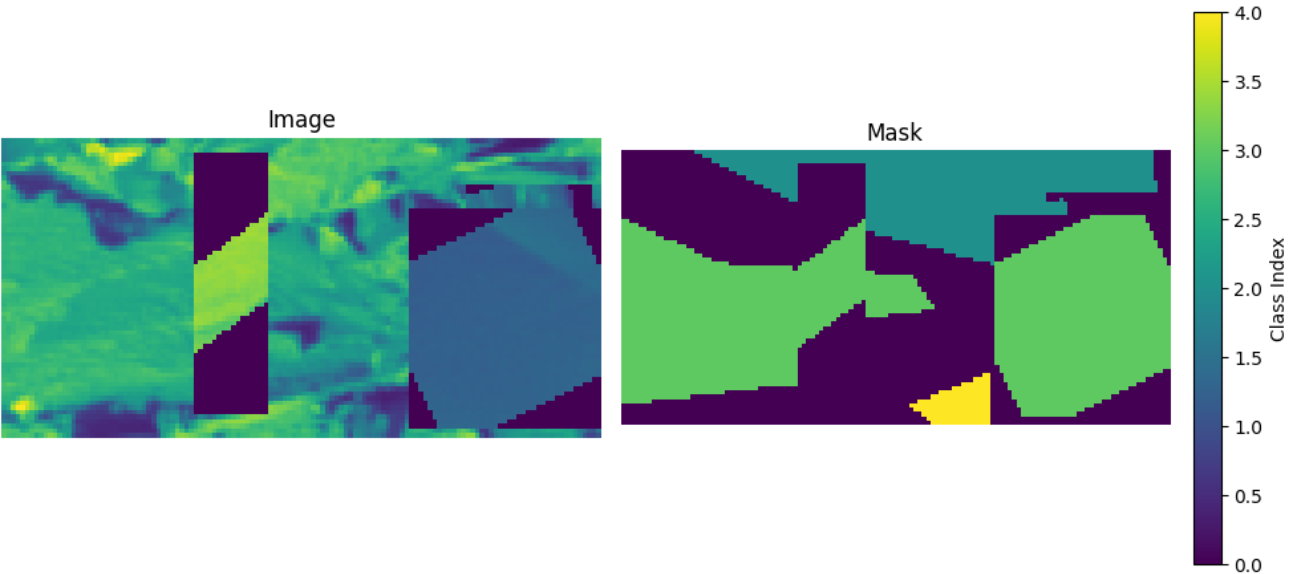
\includegraphics[width=0.45\textwidth]{reports/images/Augmented_image_mask.png}
            \caption{\small Mid-training prediction}
        \end{figure}
        
        \subsection{UNet architecture}
        
        The main model architecture used was a custom UNet model, utilizing an encoder-decoder structure with skip connections to preserve spatial information. 
        This architecture enabled the model to extract hierarchical features and make pixel-wise predictions. 
        The training we made was made almost every time on the augmented dataset.

        \begin{figure}[H]
            \centering
            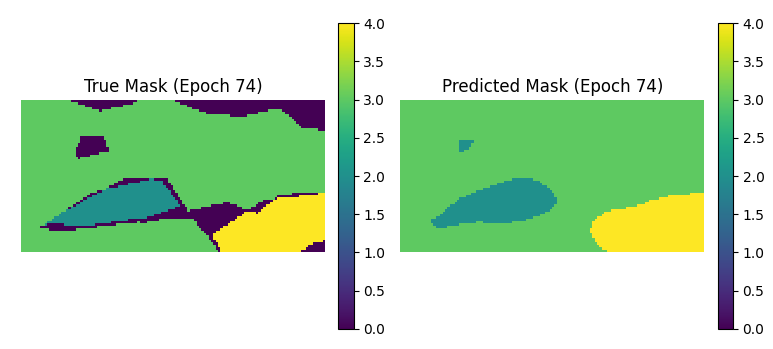
\includegraphics[width=0.45\textwidth]{reports/images/prediction1.png}
            \caption{\small Mid-training prediction}
        \end{figure}
        
        \subsection{Loss function exploration}
        
        We experimented with various loss functions during the training phase.
        We started with a \textit{categorical cross-entropy}, for later exploring a \textit{dice loss} and a {mean intersection over union loss}.
        Moreover, we also opted for combining losses together hoping to find better compromises and therefore better results.
        In the end, the \textit{focal loss} was the best scoring alternative; we also exploited the \textit{class weights} implementation of this loss function, which massively helped the model focus on smaller classes like {big rock} while ignoring the background class and improving both global and local segmentation accuracy and MIOU.
        
        \section{Experiments}
        
        \subsection{Model architecture adjustments}
        
        The layers of out UNet model architecture were fine tuned during the training process.
        By adjusting the number of convolutional layers, filter sizes, and kernel depths, feature extraction improved, and pixel-wise predictions got more distincts.
        These adjustments helped the model capture more complex terrain features.

        Training was conducted on Colab\cite{colab2024} and Kaggle\cite{kaggle2024} GPUs
        The TensorFlow\cite{tensorflow2015} Keras\cite{keras2015} and PyTorch\cite{pytorch2019} frameworks were also utilized during model development and training.

        To get an idea of the training metrics evolution, here after we present a table with the values corresponding to some models throughout the experimentation phase.

        \begin{table}[H]
            \centering
            \small
            \begin{tabular}{|c|c|c|}
                \hline
                \multicolumn{3}{|c|}{\textbf{Mean IoU}} \\ \hline
                \textbf{Model Name} & \textbf{Local} & \textbf{Submission} \\ \hline
                \multicolumn{3}{|c|}{\textbf{Early Stage Models}} \\ \hline
                UNet & 0.43 & 0.44  \\ \hline
                UNet ResNet34 & 0.60 & 0.43 \\ \hline
                \multicolumn{3}{|c|}{\textbf{Middle Stage Models}} \\ \hline
                UNet & 0.47 & 0.52 \\ \hline
                UNet squeeze \& excitement & 0.66 & 0.57 \\ \hline
                \multicolumn{3}{|c|}{\textbf{Late Stage Models}} \\ \hline
                DeepLabV3Plus & 0.61 & 0.69 \\ \hline
                SegFormer & 0.63 & \textbf{0.74} \\ \hline
            \end{tabular}
            \caption{Metrics throghout training}
        \end{table}
        
        \subsection{Advanced architectures}
        
        We also explored more advanced architectures. One such architecture was a dual UNet model, which combined the outputs of two parallel UNet networks. Another enhancement involved the incorporation of squeeze-and-excite blocks, which improve the model's ability to recalibrate channel-wise feature responses. We also experimented with transformer-based architectures, which excel at capturing long-range dependencies. Furthermore, residual blocks were integrated to improve gradient flow and prevent overfitting, ultimately boosting the model's learning capacity.

        \section{Conclusions}
        \subsection{Final Model}
        For the final submission, we employed a well-established and reliable architecture known as "Segformer." This model leverages the power of self-attention mechanisms to efficiently capture both local and global dependencies within the input data, which is particularly beneficial for segmentation tasks. Given the relatively small size of our dataset, we initially began with a lightweight configuration, progressively increasing the model complexity while carefully monitoring the risk of overfitting. This approach allowed us to balance model performance with generalization.
        
        The model was trained using a 10,000-sample augmented training set and evaluated on a separate 1,000-sample augmented validation set, providing a more robust assessment of its performance. The optimizer used was AdamW with a weight decay of 1e-3 and gradient clipping set to a norm of 1.0, ensuring stable training. Due to the diverse nature of the augmented data, a batch size of 32 was selected to maintain a good trade-off between memory efficiency and model convergence. Callbacks like model checkpoints, early stopping and LRSchedulers were employed, leading to a training session of 100 epochs on average. 
        
        For the final iteration of Segformer, we utilized the 'timm\-regnetx\_160' encoder, with a depth of 5 and 256 channels in the decoder block. This choice of encoder was driven by its ability to balance model efficiency and expressive power, making it well-suited for the task at hand. The implementation of this model was facilitated by the Segmentation Models library\cite{qubvel2024}, which provides a framework for building segmentation networks.

        The local benchmark yielded a MIOU of \textbf{0.631}, and a online evaluation of \textbf{0.740}.        \subsection{Contribution}

        Experimentation and training tasks were carried out equally and coordinately by each team member.
        Everyone mainly focused on a specific objective, as follows.
        Alibeaj worked on the development and implementation of the UNet architecture.
        Bettiati focused on refining and optimizing the UNet model for better performance.
        Bianchi investigated and experimented with various loss functions to improve segmentation accuracy.
        Ostidich led the data augmentation efforts, applying various transformations to enhance model generalization.

        \bibliographystyle{abbrv}
        \bibliography{reports/references}

    \end{multicols}
\end{document}